\documentclass{article}
\usepackage[utf8]{inputenc}
\usepackage{graphicx}
\usepackage{hyperref}
\usepackage{mathtools}
\usepackage[noabbrev,nameinlink]{cleveref}

\usepackage[style=apa]{biblatex} 
\addbibresource{bibliography.bib}


\title{RL\_Proyect}
\author{Carlos Soto (carlos.soto362@gmail.com)}
\date{June 2022}

\begin{document}

\maketitle

\section{Pure exchange with two commodities and two consumers or a Edgeworth box economy}
\textit{This section is based on \cite{mas-colell}}.\\
Pure exchange means no production. The simplest economy with profitable exchange with no production is the one with two commodities and two consumers. No production for this economy means that, the total amount of good $l$ that each of the consumers posses is less or equal than the initial amount of the good, with equality when there is no consumption and no waste. Denoting by $\{A,B\}$ the consumers, $x_{il}$ the total amount of good $l$ that consumer $i$ posses, $w_{il}$ the endowments, the initial amount of good $l$ that consumer $i$ posses and $\bar{w}_l$ the total amount of good $l$, no production, no consumption and no waste is represented by the equation,
\begin{equation}
\label{feasible}
    x_{Al} + x_{Bl} = w_{Al} + w_{Bl} = \bar{w}_l.
\end{equation}

The two tuples $\{(x_{A1},x_{A2}),(x_{B1},x_{B2})\}$ are called an ``Allocation'', all the Allocations that obey \cref{feasible} are called feasible allocations. Given a set of prices $(p_1,p_2)$, each consumer can exchange their initial goods with the budget constrain
\begin{equation}
    \label{budget}
    p_1x_{i1} + p_2x_{i2} = p_1w_{i1} + p_2w_{i2}.
\end{equation}
The consumers are going to exchange their goods in order to maximise their utility function $u_i(x_{i1},x_{i2})$. This is a function that describes the level of happiness that the consumer fills given an allocation. 

All the feasible allocations in this economy can be represented in the \textit{Edgeworth box} \cref{box1}, where the amount of good 1 that consumer $A$ posses is represented in the $x$ axis, and the amount of good 2 that consumer $A$ posses in the $y$ axis in the usual form, while the same applies for consumer $B$ but with the origin in the opposite corner. 

Given a utility function $u_A(x_{A1},x_{A2})$, a set of prices $(p_1,p_2)$ and an initial endowment $(w_{A1},w_{A2})$, there exist a feasible allocation such that the consumer $A$ maximise his utility function subject to his budget constrain. For an arbitrary set of prices, this allocation is different from the allocation that maximises $u_B(x_{B1},x_{B2})$. A Walraisan or competitive equilibrium for the Edgeworth box economy is a price vector $p^*$ and an Allocation, such that both utility functions are maximised under their respective budget constrains. 

\begin{figure}
    \centering
    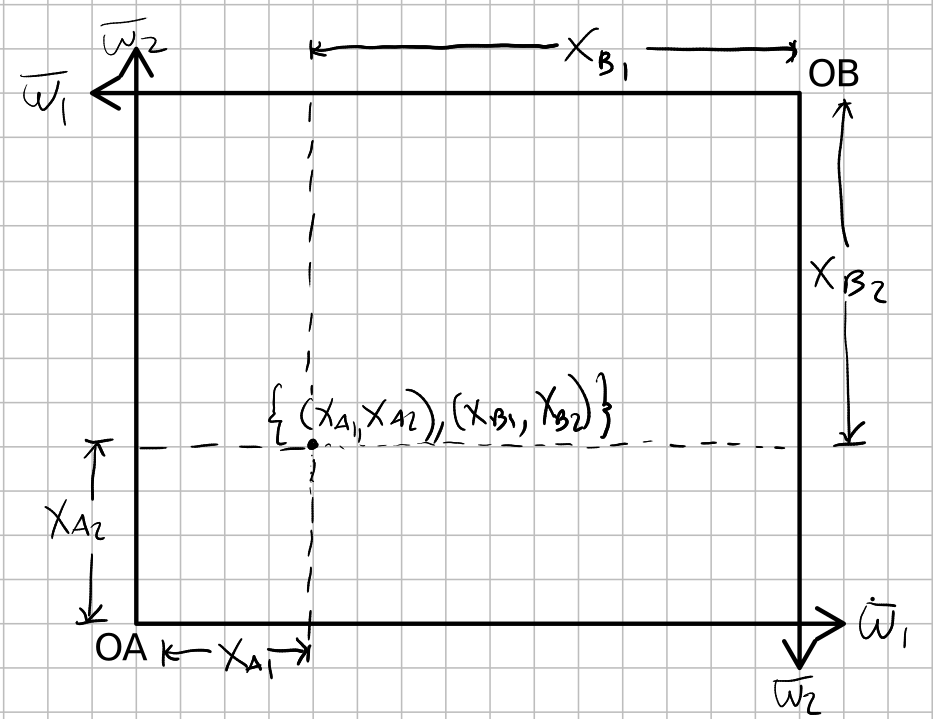
\includegraphics[scale=0.25]{box1.png}
    \caption{Representation of the Edgeworth box, where one feasible allocation has been remarked.}
    \label{box1}
\end{figure}


\section{Translating the Edgeworth box economy to a Reinforcement Learning problem}

The Edgeworth box economy can be understood as a game, where two consumers exchange two goods, in order to maximise their utility function. Under complete knowledge of the utility functions, total amount of each good and initial endowments, it is possible to find the competitive equilibrium, so, under rationality assumptions, we could assume that the consumers would agree on the price of the goods as the price of this equilibrium, and exchange the necessary amount in order for they to maximise their utility function. However, this is far away from reality. Consumers rarely know how is the total amount of each good, the utility function of the other consumers and in most of the cases, they don't know their own utility function. This can be translated as a reinforcement learning (RL) problem with no knowledge of the world. 
\subsection*{Elements of the RL problem}
\subsubsection*{World}
The world consist of the utility functions of each consumer $u_A(x_{A1},x_{A2})$,\\ $u_B(x_{B1},x_{B2})$, and the set of all possible allocations and prices \\$\{ (x_{A1},x_{A2}),(x_{B1},x_{B2}),(p1,p2) \}$ such that \cref{feasible} is obeyed. 

To be able to work with the methods of reinforcement learning, this world is going to be discretized in the following manner,

for $n_1,n_2 \in \mathbf{N}$ , defined $\eta_1 = \bar{w}_1/n_1$,  $\eta_2 = \bar{w}_2/n_2$. Then, $p_1 = 1$, $p_2 \in \{\eta_2/\eta_1,2\eta_2/\eta_1, \hdots , \bar{w}_2/\eta_1 , \eta_2/2\eta_1,\hdots,\eta_2/\bar{w}_1 \}$, $x_{i1} \in \{\bar{w}_1,\bar{w}_1 - \eta_1 ,\hdots,0 \}$ and $x_{i2} \in \{\bar{w}_2,\bar{w}_2 - \eta_2 ,\hdots,0 \}$.

This discretisation transforms the Edgeworth box in a three dimensional greed world with $(n_1+1)(n_2+1)(n_1+n_2 + 1)$ points. The price $p_1$ can be set to one because what determines the competitive equilibrium is the ration between the two prices.

In this world, there is only one point where equilibrium can be reached. 

\subsubsection*{Actions}
Without knowledge of their utility function, each consumer can only see the reward (the value of the utility function) after they have change the allocation. For doing so, they need to exchange with the other consumer. In order to work with this world in a similar manner than the greed world, each consumer can decide to buy or sell moving their allocation horizontally or vertically, but the movement is done only if both of the consumers agree on this decision. This agreement will be done in the following way:

If a consumer decide to sell an amount of good 2 according to his policy in the present point, he needs also to decide if he want to sell at the same, increase or decrease price, moving the state up or down in the price direction. Next, if the other customer decides to buy according to the policy evaluated in the original point, then she needs to see if she still wants to buy according to her policy evaluated in the new point, if the result is affirmative and if the price is affordable (is less that her budget evaluated in the current point), then they exchange giving the equivalent amount of good 1 in exchange of the amount of good 2. If the other customer don't want to buy according to her policy in the new point, then nothing happens, and the point returns to the original place. 

If both customers want to buy the good 2, nothing happens. If both customers want to sell the good 2, nothing happens.  

Summarizing, the actions for each customer can be, buy good 2, selling good 2 at the same price, selling good 2 with increase price and selling good 2 with decreased price. 

\subsubsection*{Rewards}
The rewards would be the value of their utility function after the action has been taken. The utility functions don't need to be the same for both customers. They are assumed to be concave functions of the goods. 

\subsection*{Possible simplification }
In case the dynamics don't manage to reach the competitive equilibrium because the learning algorithm is not well fitted for this problem or the problem is to big, one possible simplification could be to make the prices fix. The fixation of the prices would make that the competitive equilibrium may not exist, so, to ensure the existence, the problem could be set to $u_A(x_{A1},x_{A2})=u_B(x_{B1},x_{B2})$, and the initial budgets to be also equal, such that the competitive equilibrium would be $\{ (1/2,1/2),(1/2,1/2),(1,1)   \}$ by symmetry. 

\printbibliography
\end{document}
